\section{Oefeningen}
\begin{oef}
\label{oef21}
$A = \{1, 3, 5, 7\}$ en  $B = \{2, 4, 6,8\}$. Noteer volgende relaties door middel van opsomming:
\begin{enumerate}
\item $U=\{(x,y) \mid x\in A \mathrm{~en~} y \in B \mathrm{~en~} x+y<9\}$
\item $V=\{(x,y) \mid x\in A \mathrm{~en~} y \in B  \mathrm{~en~} x<y \}$
\end{enumerate}
\begin{opl}
\begin{enumerate}
\item $U=\{(1,2),(1,4),(1,6),(3,2),(3,4),(5,2) \}$
\item $V=\{(1,2),(1,4),(1,6),(1,8),(3,4),(3,6),(3,8),(5,6),(5,8),(7,8) \}$
\end{enumerate}
\end{opl}
\end{oef}

\begin{oef}
\begin{enumerate}
\item Bepaal domein en bereik van de relaties van oefening~2.1.
\item Geef de meest correcte benaming van de relaties.
\end{enumerate}
\begin{opl}
\begin{enumerate}
\item $\dom{U}=\{1,3,5 \}$; $\range{U}=\{2,4,6 \}$; relatie, geen injectie (want bvb. in het element 2 komen drie pijlen toe) of surjectie (want in het element 8 komt geen pijl toe). De relatie is geen functie want er zijn elementen met meer dan \'e\'en beeld (bvb. het element 1 heeft drie beelden).
\item $\dom{V}=\{1,3,5,7 \}$; $\range{V}=\{2,4,6,8 \}$; surjectieve relatie
\end{enumerate}
\end{opl}
\end{oef}




\begin{oef}
Gegeven $X = \{\mathrm{a},\mathrm{ b}\}$ en $Y = \{\mathrm{c}, \mathrm{d}, \mathrm{e}, \mathrm{f}\}$. Noteer volgende productverzamelingen door middel van opsomming:
\begin{enumerate}
\item $X\times Y$
\item $Y\times X$
\item $X^2$
\end{enumerate}
\begin{opl}
\begin{enumerate}
\item $X\times Y=\{(a,c),(a,d),(a,e),(a,f),(b,c),(b,d),(b,e),(b,f) \}$
\item $Y\times X=\{(c,a),(c,b),(d,a),(d,b),(e,a),(e,b),(f,a),(f,b) \}$
\item $X^2=\{(a,a),(a,b),(b,a),(b,b) \}$
\end{enumerate}
\end{opl}
\end{oef}

\begin{oef}
Een e-mailadres kan je beschouwen als  een productverzameling van drie verzamelingen. Noteer deze verzamelingen zorgvuldig en definieer de gevraagde productverzameling.
\begin{opl}
$A=\{\text{strings bestaande uit a-zA-Z,.,0-9} \}$\\
$B=\{\text{strings bestaande uit a-zA-Z,.} \}$\\
$C=\{ \text{strings uit de lijst met goedgekeurde TLD's (Top Level Domain names}\}$\\
$A\times B\times C$
\end{opl}
\end{oef}

\begin{oef}
Hieronder vind je een aantal relaties van verzameling $A$ naar $B$. 
\begin{itemize}
\item Definieer voor elk van de gevallen de verzamelingen $A$ en $B$ eenduidig. Er zijn verschillende mogelijkheden.
\item Zoek een gepaste voorstellingswijze voor de relatie
\item Bepaal  welk soort relatie er beschreven wordt.
\end{itemize}
\begin{enumerate}
\item Klant heeft contactmoment
\item Klant heeft id
\item Persoon woont op adres
\item Student heeft telefoonnummer
\item Student krijgt rapport
\item Student volgt OPO
\end{enumerate}
\begin{opl}
\begin{enumerate}

\item Klant heeft contactmoment: $A$=$\{\text{klanten van het bedrijf}\}$; \\
$B=\{\text{mogelijke contactmomenten voor manager}\}$; 
\'e\'en klant kan meerdere contactmomenten hebben, maar is er niet toe verplicht; 
niet alle mogelijke contactmomenten moeten ingevuld worden, maar nooit meer dan \'e\'en klant per contactmoment: injectieve relatie

\item Klant heeft id: $A$=$\{\text{klanten van het bedrijf}\}$; \\
$B=\{\text{id's die de software toegekend heeft}\}$ 
iedere klant heeft juist \'e\'en id: bijectie (afbeelding die bijectief is)

\item Persoon woont op adres: $A=\{\text{mensen met een geregistreerd adres}\}$; \\
$B=\{\text{geregistreerde adressen}\}$; iedere persoon woont op \'e\'en adres; op \'e\'en adres kunnen meerdere personen wonen: surjectie (afbeelding die surjectief is); als $A$ ook daklozen bevat: surjectieve functie

\item Student heeft telefoonnummer: $A=\{\text{studenten KHLeuven}\}$; \\
$B=\{$telefoonnummers die in het studentenregistratiesysteem opgenomen zijn$\}$.  Iedere student heeft nul, \'e\'en of meerdere telefoonnummers; ieder telefoonnummer heeft \'e\'en eigenaar: bijectieve relatie.
Als je broers en zussen toelaat als student: surjectieve relatie want telefoonnummer kan horen bij verschillende studenten.

\item Student krijgt rapport: $A=\{\text{leerlingen van KHLeuven}\}$; \\
$B=\{\text{afgedrukte rapporten op het einde van een examenperiode}\}$ voor elke student is er juist \'e\'en rapport: bijectie (afbeelding die bijectief is)

\item Student volgt OPO: $A=\{\text{studenten van KHLeuven}\}$; \\
$B=\{\text{OPO's die de KHLeuven inricht}\}$ student volgt meerdere OPO's en elk OPO wordt door meerdere studenten gevolgd: surjectieve relatie, tenzij er OPO's zijn die door geen enkele student gevolgd worden (dat zou kunnen gebeuren bij keuzeOPO's bvb). In dat geval is het een gewone relatie.
\end{enumerate}

\end{opl}
\end{oef}

\begin{oef}\label{oef:26}
Definieer volgende relaties correct:
\begin{itemize}
  \item Bepaal bron- en doelverzameling zodat de relatie een bijectie is.
  \item Stel de relatie voor als een verzameling van paren door middel van een functievoorschrift, bijv.\ $U=\{(x,y)|x,y\in \real\text{ en } y=x+1\}$
  \item Geef nog minstens \'e\'en andere voorstellingswijze
\end{itemize}
\begin{enumerate}
  \item de functie $y=\sqrt{x}$
  \item de relatie die de kostprijs van de brandstof van een autorit weergeeft
        in functie van de lengte van de rit (uitgedrukt in kilometers). De auto
        verbruikt \SI{6,45}{\litre} per \SI{100}{\kilo\meter}. De brandstof kost \euros{1,315} per liter.
  \item de relatie die de prijs van de factuur van een mazoutlevering weergeeft
        in functie van het aantal gekochte liter. Mazout kost \euros{0,9155} per
        liter als je minder dan \SI{2000}{\litre} afneemt en \euros{0,8887}
        per liter als je meer dan \SI{2000}{\litre} afneemt.
\end{enumerate}
\begin{opl}
\begin{enumerate}
  \item \begin{enumerate}
          \item bron- en beeldverzameling: $\real^+$
          \item $U=\{(x,y)|x,y\in \real^+\text{ en } y=\sqrt{x} \}$
          \item zie figuur~\ref{oef:opl26}
                \begin{figure}[htbp]
                  \centering
                  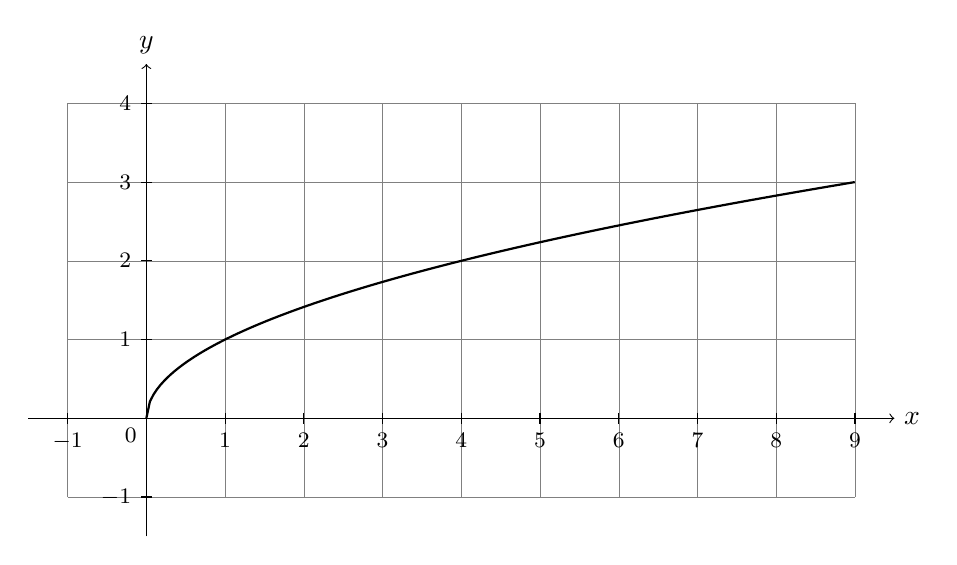
\begin{tikzpicture}[x=1cm,y=1cm]
                  \draw[help lines] (-1,-1) grid (9,4);
                  \draw[->] (-1.5,0) -- (9.5,0) node[right] {$x$};
                  \draw[->] (0,-1.5) -- (0,4.5) node[above] {$y$};
                  \foreach \x in {-1,1,2,...,9}
                          \draw[shift={(\x,0)}] (0pt,2pt) -- (0pt,-2pt) node[below] {\footnotesize $\x$};
                  \foreach \y in {-1,1,2,...,4}
                          \draw[shift={(0,\y)},color=black] (2pt,0pt) -- (-2pt,0pt) node[left] {\footnotesize $\y$};
                  \draw [domain=0:9,samples=200,thick] plot(\x,{sqrt(\x)});
                  \node [below left] at (0,0) {\footnotesize 0};
                  \end{tikzpicture}
                  \caption{Oplossing van oefening~\ref{oef:26}}\label{oef:opl26}
                \end{figure}
        \end{enumerate}
  \item \begin{enumerate}
          \item bron- en beeldverzameling is  $\real^+$
          \item $U=\{(x,y)|x,y\in \real^+\text{ en } y=8,48175\cdot x/100\}$
        \end{enumerate}
  \item \begin{enumerate}
          \item bron- en beeldverzameling is  $\real^+$
          \item $U = \left\lbrace (x,y)\;|\; x,y \in \real^+
                \text{ en } y = \begin{cases}
                                  0,9155\cdot x&\text{ als }x<2000\\
                                  0,8887\cdot x&\text{ anders }
                                \end{cases} \qquad \right\rbrace$
        \end{enumerate}

\end{enumerate}
\end{opl}
\end{oef}

\begin{oef}
Wat is de inverse van volgende relaties? Stel de relatie voor op dezelfde manier als de opgave.
\begin{enumerate}
  \item $\{(1,7),(2,10),(3,9) \}$
  \item \begin{tabular}{c|cccccc}
          $x$ & \num{0.1} & \num{0.2} & \num{0.3} & \num{0.4} & \num{0.5} & \num{0.6} \\ 
          \midrule
          $y$ & 2 & 4 & 6 & 8 & 10 & 12 \\ 
        \end{tabular} 
  \item $f: \real\rightarrow\real:x\mapsto y \mid y=2\cdot x+10 $
  \item $f: \real^+\rightarrow\real:x\mapsto y \mid y=\sqrt{x}$
\end{enumerate}
\begin{opl}
\begin{enumerate}
  \item \{(7,1),(10,2),(9,3) \}
  \item \begin{tabular}{c|cccccc}
          $y$ & 2 & 4 & 6 & 8 & 10 & 12 \\ 
          \midrule
          $x$ & \num{0.1} & \num{0.2} & \num{0.3} & \num{0.4} & \num{0.5} & \num{0.6} \\ 
        \end{tabular} 
  \item $f^{-1}: \real\rightarrow\real:x\mapsto  y=\dfrac{x-10}{2} $
  \item $f^{-1}: \real^+\rightarrow\real^+:x\mapsto y=x^2$
\end{enumerate}
\end{opl}
\end{oef}



\begin{oef}
Zelfde vraag voor elke figuur:
\begin{itemize}
  \item Teken de inverse functie.
  \item Wat is het functievoorschrift van de getekende functie en zijn inverse?
\end{itemize}
\begin{enumerate}
  \begin{minipage}{\columnwidth}
    \item 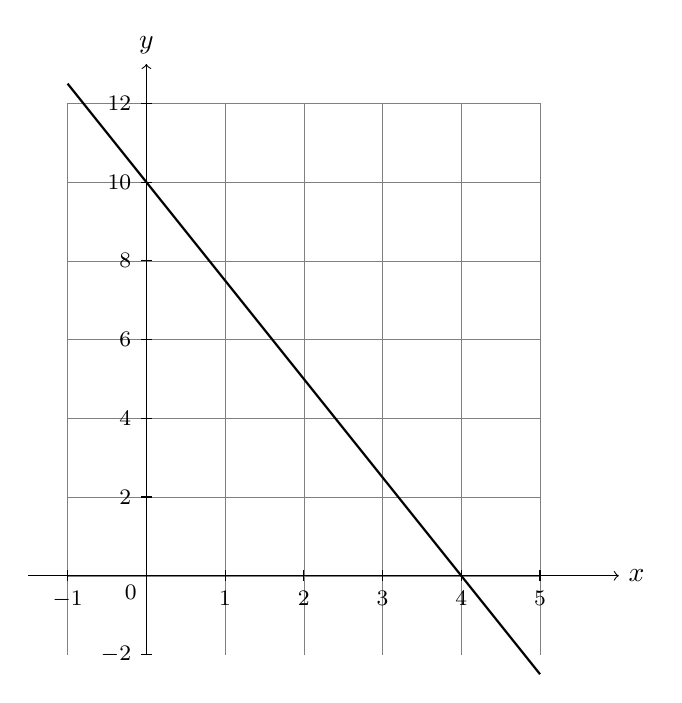
\begin{tikzpicture}[x=1cm,y=.5cm]
            \draw[help lines] (-1,-2) grid (5,12);
            \draw[->] (-1.5,0) -- (6,0) node[right] {$x$};
            \draw[->] (0,-2) -- (0,13) node[above] {$y$};
            \foreach \x in {-1,1,2,...,5}
                    \draw[shift={(\x,0)}] (0pt,2pt) -- (0pt,-2pt) node[below] {\footnotesize $\x$};
            \foreach \y in {-2,2,4,...,12}
                    \draw[shift={(0,\y)},color=black] (2pt,0pt) -- (-2pt,0pt) node[left] {\footnotesize $\y$};
            \draw[thick](5,-2.5) -- (-1,12.5); % rechte 1
            \node [below left] at (0,0) {\footnotesize 0};
          \end{tikzpicture}
  \end{minipage}
  \begin{minipage}{\columnwidth}
    \item 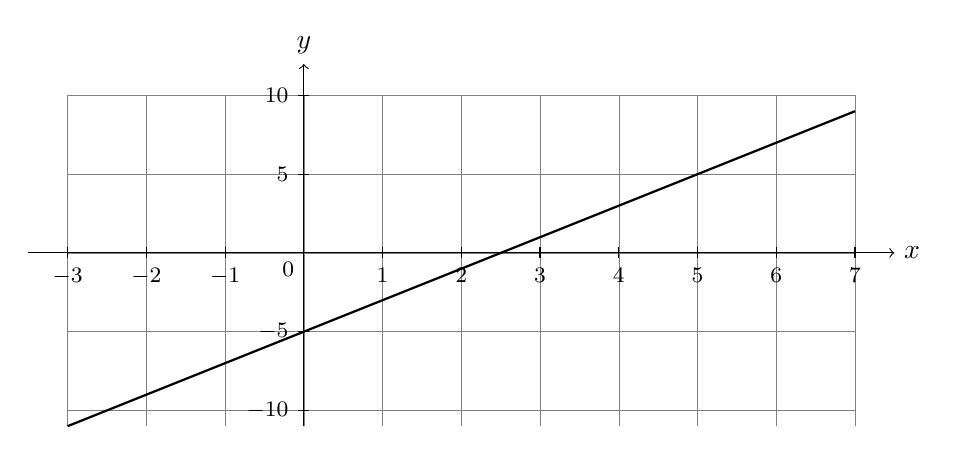
\begin{tikzpicture}[x=1cm,y=.2cm]
            \draw[help lines] (-3,-11) grid (7,10);
            \draw[->] (-3.5,0) -- (7.5,0) node[right] {$x$};
            \draw[->] (0,-11) -- (0,12) node[above] {$y$};
            \foreach \x in {-3,-2,-1,1,2,...,7}
                    \draw[shift={(\x,0)}] (0pt,2pt) -- (0pt,-2pt) node[below] {\footnotesize $\x$};
            \foreach \y in {-10,-5,5,10}
                    \draw[shift={(0,\y)},color=black] (2pt,0pt) -- (-2pt,0pt) node[left] {\footnotesize $\y$};
            \draw[thick](-3,-11) -- (7,9); % rechte 1
            \node [below left] at (0,0) {\footnotesize 0};
          \end{tikzpicture}
  \end{minipage}
  \begin{minipage}{\columnwidth}
    \item 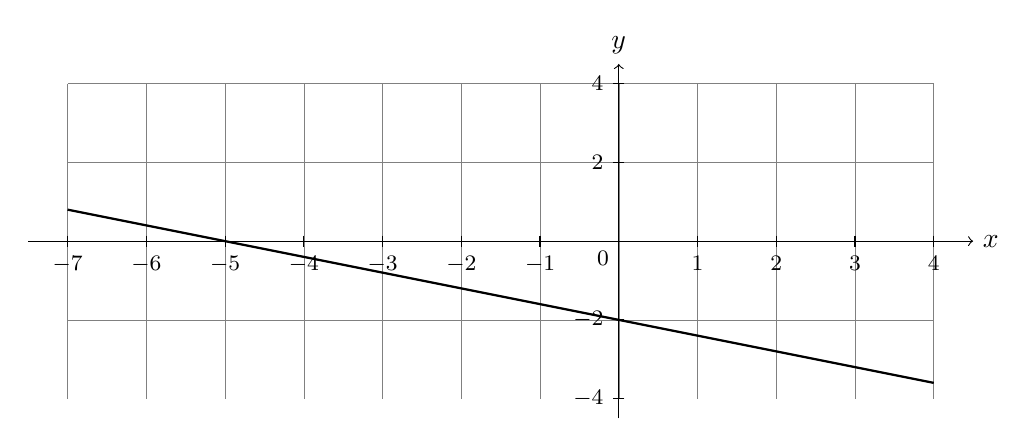
\begin{tikzpicture}[x=1cm,y=.5cm]
            \draw[help lines] (-7,-4) grid (4,4);
            \draw[->] (-7.5,0) -- (4.5,0) node[right] {$x$};
            \draw[->] (0,-4.5) -- (0,4.5) node[above] {$y$};
            \foreach \x in {-7,-6,...,-1,1,2,...,4}
                    \draw[shift={(\x,0)}] (0pt,2pt) -- (0pt,-2pt) node[below] {\footnotesize $\x$};
            \foreach \y in {-4,-2,2,4}
                    \draw[shift={(0,\y)},color=black] (2pt,0pt) -- (-2pt,0pt) node[left] {\footnotesize $\y$};
            \draw[thick](-7,0.8) -- (4,-3.6); % rechte 1
            \node [below left] at (0,0) {\footnotesize 0};
          \end{tikzpicture}
  \end{minipage}
\end{enumerate}

\begin{opl}
\begin{enumerate}
\item $y=-\frac52 x +10$; inverse functie: $y=-\frac25 x +4$
\item $y=2x-5$; inverse functie: $y=\frac12 x+\frac52$
\item $y=-\frac25x-2$; inverse functie: $y=-\frac52x-5$
\end{enumerate}
\end{opl}
\end{oef}



\begin{oef}
De volgende grafieken stellen relaties voor met als bron- en doelverzameling het interval $[0,1]$. Geef voor elk van de relaties aan of deze
functies, afbeeldingen, injectief, surjectief en/of bijectief zijn.
\begin{center}
  \newcommand{\axes}{
    \path[use as bounding box] (-.5,-.5) rectangle (4,4);
    \draw[step=3cm,gray,thin] (-.5,-.5) grid (4,4);
    \draw[thin,->] (-.5,0) -- (4,0);
    \draw[thin,->] (0,-.5) -- (0,4);
  }
  \begin{tabular}{cc}
    1.
    \begin{tikzpicture}
      \axes
      \draw[thick] (0,0) -- (3,3);
    \end{tikzpicture}
    &
    2.
    \begin{tikzpicture}
      \axes
      \draw[thick] (0,0) to[out=90,in=-90] (3,3);
    \end{tikzpicture}
    \\
    3.
    \begin{tikzpicture}
      \axes
      \draw[thick] (1.5,0) -- (1.5,3);
    \end{tikzpicture}
    &
    4.
    \begin{tikzpicture}
      \axes
      \draw[thick] (0,1.5) -- (3,1.5);
    \end{tikzpicture}
    \\
    5.
    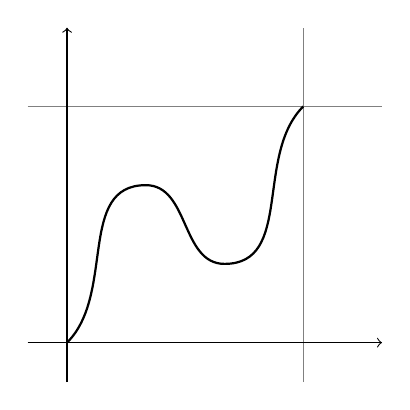
\begin{tikzpicture}
      \axes
      \draw[thick] (0,0) to[out=45,in=180] (1,2) to[out=0,in=180] (2,1) to[out=0,in=225] (3,3);
    \end{tikzpicture}
    &
    6.
    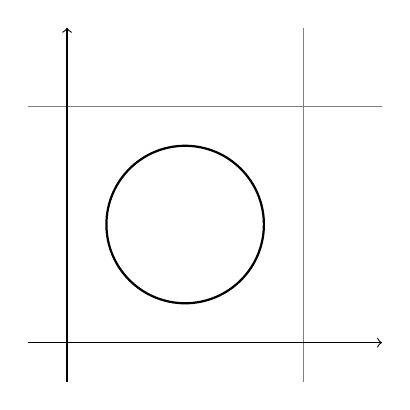
\begin{tikzpicture}
      \axes
      \draw[thick] (1.5,1.5) circle (1cm);
    \end{tikzpicture}
  \end{tabular}
\end{center}
\begin{opl}
  \hspace{1mm}
  \begin{center}
    \begin{tabular}{cccccc}
      & \rotatebox{90}{functie}
      & \rotatebox{90}{afbeelding}
      & \rotatebox{90}{injectief}
      & \rotatebox{90}{surjectief}
      & \rotatebox{90}{bijectief} \\
      \toprule
      1. & \checkmark & \checkmark & \checkmark & \checkmark & \checkmark \\
      2. & \checkmark & \checkmark & \checkmark & \checkmark & \checkmark \\
      3. &            &            &            &            &            \\
      4. & \checkmark & \checkmark &            &            &            \\
      5. & \checkmark & \checkmark &            & \checkmark &            \\
      6. &            &            &            &            &            \\
    \end{tabular}
  \end{center}
\end{opl}
\end{oef}

%%% Local Variables: 
%%% mode: latex
%%% TeX-master: "../cursusTW1"
%%% End: 
